\documentclass[a4paper]{report}

\usepackage{times}
\usepackage{graphicx}
\usepackage{wrapfig}
\usepackage{pdfpages}
\usepackage{hyperref}
\usepackage{fancyheadings}

\hypersetup{
  colorlinks=true,
  linkcolor=black
  }
  
\def\topfraction{.9}
\def\bottomfraction{.9}
\def\textfraction{.1}
\def\floatpagefraction{.9}

\setlength{\parindent}{0mm}
\usepackage{parskip}
\usepackage{color}
\usepackage{sectsty}
\allsectionsfont{\sffamily}
\makeatletter
\newcommand\funcsection{%
\@startsection{section}{1}{\z@}%
  {-3.5ex \@plus -1ex \@minus -.2ex}%
  {2.3ex \@plus.2ex}%
  {\color{red}\sffamily\huge\bfseries}}
\makeatother

\input{release.tex}

\usepackage{fancyvrb}
\fvset{formatcom=\color{blue},fontseries=c,fontfamily=courier,xleftmargin=4mm,commentchar=!}
\DefineVerbatimEnvironment{Code}{Verbatim}{formatcom=\color{blue},fontseries=c,fontfamily=courier,fontsize=\footnotesize,xleftmargin=4mm,commentchar=!}

\pagestyle{empty}

\def\Mlab{MATLAB$^{\textsuperscript{\textregistered}}$}

\begin{document}
\includepdf{titlepage}
\thispagestyle{empty}
\newpage
\vspace*{\fill}
\begin{tabular}{ll}
Release & \release \\
Release date & \reldate \\[20pt]
Licence & LGPL \\
Toolbox home page &  \url{http://www.petercorke.com/robot} \\
Discussion group & \url{http://groups.google.com.au/group/robotics-tool-box}
\end{tabular}
\vspace*{\fill}
\hrule
Copyright \textcopyright 2012 Peter Corke\\
peter.i.corke$@$gmail.com\\
\url{http://www.petercorke.com}
\newpage
\vspace*{\fill}
\setlength{\fboxsep}{10pt}%

\pagestyle{headings}        % Gives page headings at top of page
\lfoot{Machine Vision Toolbox for \Mlab}
\rfoot{Copyright \copyright Peter Corke 2011}

\newpage
\setcounter{section}{0}
\addcontentsline{toc}{section}{Introduction}

\chapter*{Preface}
\pagestyle{fancyplain}
\begin{wrapfigure}{l}{4.5cm}
\vspace{-2ex}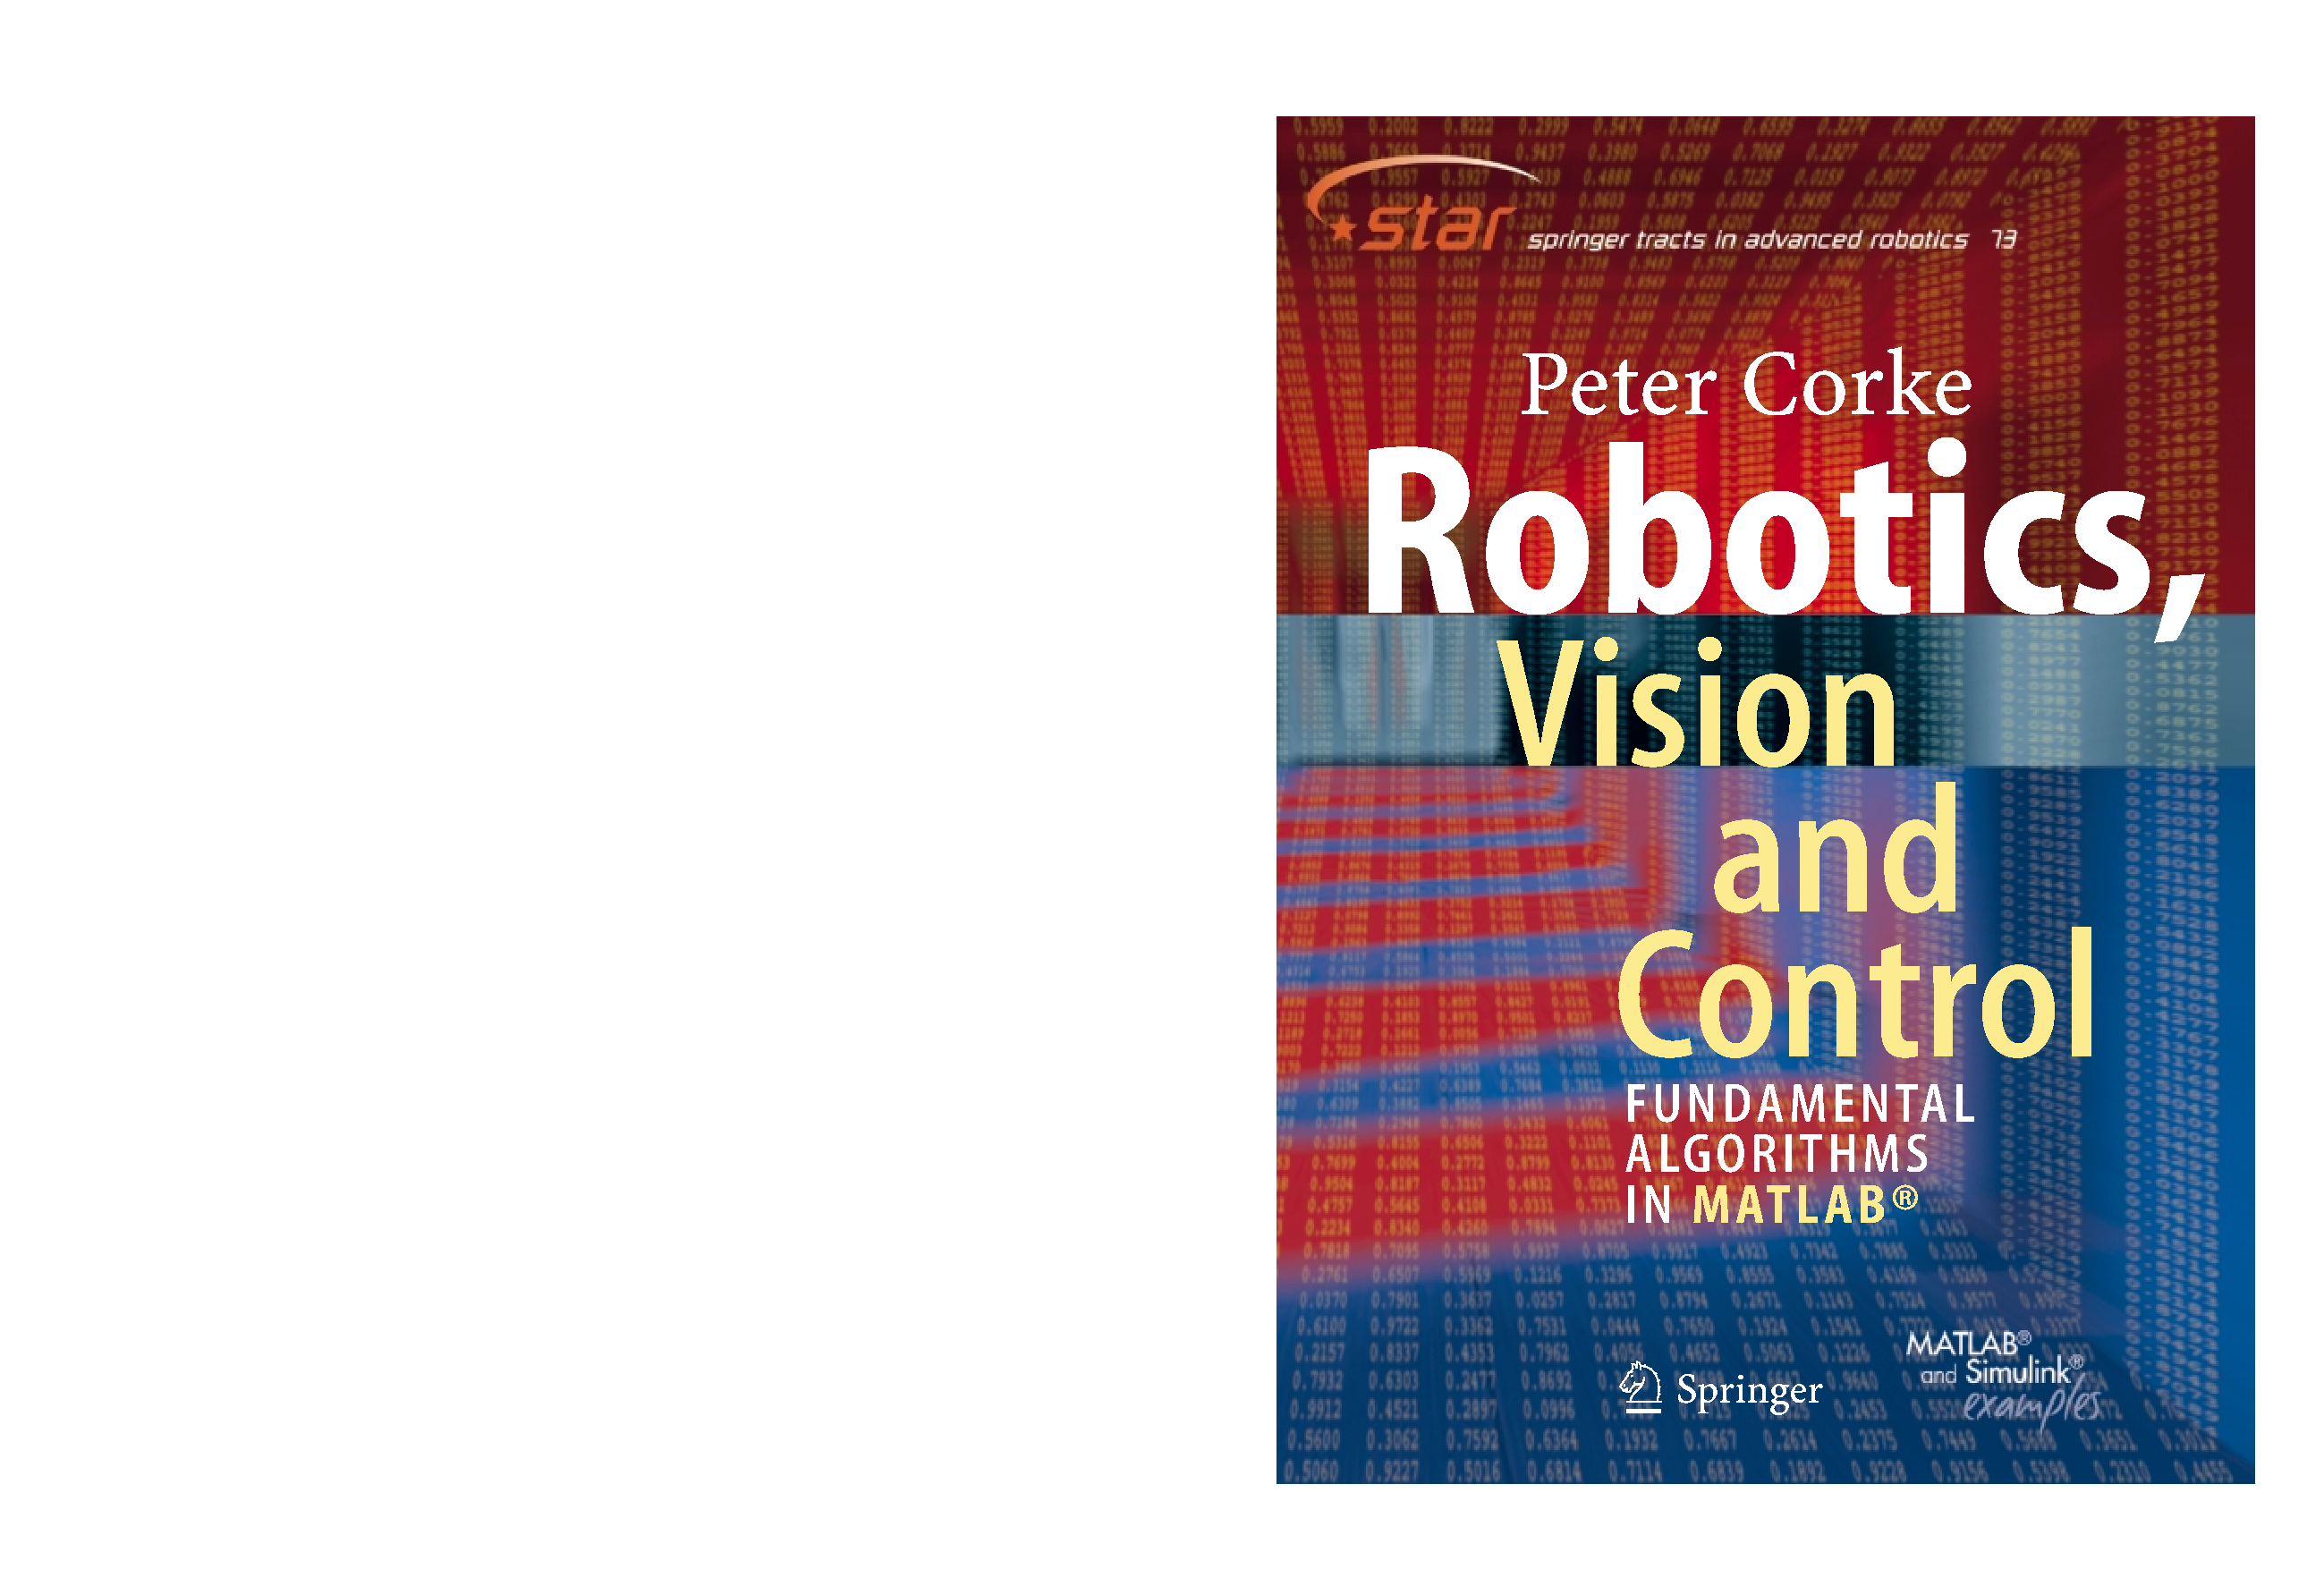
\includegraphics[width=4cm]{frontcover.pdf}
\end{wrapfigure}
This, the third release of the Toolbox, represents a decade of %% CHANGE
development.
The last release was in 2005 and this version captures a large number of changes over that period but with extensive work
over  the last two years
to support my new book ``\textit{Robotics, Vision \& Control}'' shown to the left.

The Machine Vision Toolbox (MVTB) provides many 
functions that 
are useful in machine vision and vision-based control.
It is a somewhat eclectic collection reflecting my personal interest in
areas of photometry, photogrammetry, colorimetry.
It includes over 100 functions spanning operations such as
image file reading and writing, acquisition, display, filtering,
blob, point and line feature extraction,  mathematical morphology, 
homographies, visual Jacobians,
camera calibration and color space conversion.
The Toolbox, combined with \Mlab\ and a modern workstation computer,
is a useful and convenient environment for investigation of machine
vision algorithms.  For modest image sizes the processing rate can
be sufficiently ``real-time'' to allow for closed-loop control.  Focus of
attention methods such as dynamic windowing (not provided) can be
used to increase the processing rate.
With input from a firewire or web camera (support provided) and 
output to a robot
(not provided) it would be possible to implement a visual servo system
entirely in \Mlab.

An image is usually treated as a rectangular array of scalar values representing
intensity or perhaps range.
The matrix is the natural datatype for \Mlab\ and thus makes the manipulation
of images easily expressible in terms of arithmetic statements in \Mlab
language.
Many image operations such as thresholding, filtering and statistics can
be achieved with existing \Mlab\ functions.
The Toolbox extends this core functionality with M-files that
implement functions and classes, and mex-files for some compute
intensive operations.
It is possible to use mex-files to interface with image acquisition
hardware ranging from simple framegrabbers to robots.
Examples for firewire cameras under Linux are provided.

The routines are written in a straightforward manner which allows
for easy understanding.  \Mlab\ vectorization has been used as much as
possible to improve efficiency, however some algorithms are not amenable
to vectorization.
If you have the \Mlab\ compiler available then this can be used to compile
bottleneck functions.
Some particularly compute intensive functions are provided as mex-files and
may need to be compiled for the particular platform.
This toolbox considers images generally as arrays of double precision
numbers.  This is extravagant on storage, though this is much less
significant today than it was in the past.

This toolbox is not a clone of the Mathwork's own Image Processing 
Toolbox (IPT) although there are many functions in common.
This toolbox predates IPT by many years, is open-source, contains many 
functions that are useful for image feature extraction and control.
It was developed under Unix and Linux systems and some functions
rely on tools and utilities that exist only in that environment.

The manual is now auto-generated from the comments in the \Mlab\ code itself which reduces the effort
in maintaining code and a separate manual as I used to --- the downside is that there are no worked examples and figures in the manual.
However the book ``\textit{Robotics, Vision \& Control}''  provides a detailed discussion (over 600 pages, nearly 400 figures and 1000 code examples)
of how to use the Toolbox functions to
solve many types of problems in robotics and machine vision, and I commend it to you.


\newpage
\tableofcontents
\newpage
\chapter{Introduction}

\section{Support}
There is no support!  This software is made freely available in the hope that you find it useful in solving whatever problems
you have to hand.
I am happy to correspond with people who have found genuine
bugs or deficiencies but my response time can be long and I can't guarantee that I respond to your email.
I am very happy to accept contributions for inclusion in future versions of the
toolbox, and you will be suitably acknowledged.

\textbf{I can guarantee that I will not respond to any requests for help with assignments or homework, no matter
how urgent or important they might be to you.  That's what your teachers, tutors, lecturers and professors are paid to do.}

You might instead like to communicate with other users via 
the Google Group called ``Robotics Toolbox'' 
\begin{quote}
\url{http://groups.google.com.au/group/robotics-tool-box}
\end{quote}
which is a forum for discussion.
You need to signup in order to post, and the signup process is moderated by me so allow a few
days for this to happen.  I need you to write a few words about why you want to join the list
so I can distinguish you from a spammer or a web-bot.

\section{How to obtain the Toolbox}
The Machine Vision Toolbox is freely available from the Toolbox home
page at 
\begin{quote}
\url{http://www.petercorke.com}
\end{quote}

The web page requests some information from you
regarding such as your country, type of organization and application.
This is just a means for me to gauge interest and to remind myself
that this is a worthwhile activity.

The files are available in zip format (.zip).  Download them all to
the same directory and then unzip them.  They
all unpack to the correct parts of a hiearchy of directories (folders)
headed by \texttt{rvctools}.

You may require one or more files, please read the descriptions carefully
before downloading.
\begin{itemize}
\item \texttt{vision-3.X.zip} This file is essential, it is the core Toolbox and contains
all the functions, classes, mex-files and Simulink models required 
for most of the RVC book.
\item \texttt{images.zip} These are the images that are used for
many examples in the RVC book.  These images are all found automatically
by the \texttt{iread()} function.
\item \texttt{contrib.zip} A small number of Toolbox functions depend on third party code which is included in this file. Please note and respect the licence conditions associated with these packages.
Those functions are: 
\texttt{igraphseg},
\texttt{imser}, and
\texttt{CentralCamera.estpose}.
\item \texttt{contrib2.zip} Additional third party code for
the functions: \texttt{isift}, and \texttt{isurf}.
Note that the code here is slightly modified version of the open-source
packages.
\item \texttt{images2.zip} This is a large file (150MB) containing the mosaic, campus, bridge-l and campus sequences which support the examples in Sections 14.6, 14.7 and 14.8 respectively.
\end{itemize}

If you already have the Robotics Toolbox installed then download
the zip file(s) to the directory above the existing \texttt{rvctools} directory
and then unzip them.
The files from these zip archives will properly interleave with the Robotics
Toolbox files.

Ensure that the folder \texttt{rvctools} is on your \Mlab\ search
path.  You can do this by issuing the \texttt{addpath} command at 
the \Mlab\ prompt.
Then issue the command \texttt{startup\_rvc} and it will add a number
of paths to your \Mlab\ search path.
You need to setup the path every time you start \Mlab\ but you can 
automate this by setting up environment variables, editing your 
\texttt{startup.m} script by pressing the ``Update Toolbox Path
Cache" button under \Mlab\ General preferences.

\subsection{Documentation}

This document {\tt vision.pdf} is a manual that describes all functions in the Toolbox.
It is auto-generated from the comments in the \Mlab\ code and is fully hyperlinked:
to external web sites, the table of content to functions, and the ``See also'' functions
to each other.

The same documentation is available online in
alphabetical order at \url{http://www.petercorke.com/MVTB/r3/html/index_alpha.html}
or by category at \url{http://www.petercorke.com/MVTB/r3/html/index.html}.

Documentation is also available via the \Mlab\ help browser, ``Machine
Vision Toolbox" appears under the Contents.

\section{MATLAB version issues}
The Toolbox has been tested under R2012a.

\section{Use in teaching}
This is definitely encouraged!
You are free to put the PDF manual (\texttt{vision.pdf} or the web-based documentation {\texttt{html/*.html} on a server for class
use.
If you plan to distribute paper copies of the PDF manual then every copy must include the first two pages (cover and licence).

\section{Use in research}
If the Toolbox helps you in your endeavours then I'd appreciate you citing the Toolbox when you publish.
The details are
\begin{verbatim}
@article{Corke05f,
    Author = {P.I. Corke},
    Journal = {IEEE Robotics and Automation Magazine},
    Title = {Machine Vision Toolbox},
    Month = nov,
    Volume = {12},
    Number = {4},
    Year = {2005},
    Pages = {16-25}
}
\end{verbatim}
or
\begin{quote}
``\textit{Machine Vision Toolbox}",\\
P.I. Corke, \\
IEEE Robotics and Automation Magazine, \\
12(4), pp 16--25, November 2005.
\end{quote}
which is also given in electronic form in the CITATION file.


\subsection{Other toolboxes}
Matlab Central \url{http://www.mathworks.com/matlabcentral} is a great resource for user contributed MATLAB code, and there are hundreds of modules available.
VLFeat \url{http://www.vlfeat.org} is a great collection of advanced computer vision algorithms for MATLAB.

\section{Acknowledgements}
Last, but not least, this release includes functions for computing image plane homographies and
the fundamental matrix, contributed by Nuno Alexandre Cid Martins of 
I.S.R., Coimbra.
RANSAC code by Peter Kovesi;
pose estimation by
Francesco Moreno-Noguer, Vincent Lepetit, Pascal Fua at the CVLab-EPFL;
color space conversions by Pascal Getreuer;
numerical routines for geometric vision by various members of the Visual Geometry Group at Oxford (from the web site of
the Hartley and Zisserman book;
the k-means and MSER algorithms by Andrea Vedaldi and Brian Fulkerson;the graph-based image segmentation software by Pedro Felzenszwalb;
and the SURF feature detector by Dirk-Jan Kroon at U. Twente.
The Camera Calibration Toolbox by Jean-Yves Bouguet is used unmodified.Functions such as SURF, MSER, graph-based segmentation and pose estimation are based on great code 
Some of the MEX file use some really neat macros that were part of the package VISTA Copyright 1993, 1994 University of British Columbia.
See the file \texttt{CONTRIB} for details.




\renewcommand{\section}{\funcsection}
%\setcounter{secnumdepth}{-1}
%\settocdepth{section}
\newpage
\chapter{Functions and classes}
\input{all}

\bibliographystyle{ieeetr}
\bibliography{strings,robot,control,dynamics,kinematics,force,grind,publist,software}
\end{document}
